
% !TEX root = allinone_main_v2.tex

\section{Homological stability}\label{sec:connectivity}

In this section, we estimate the connectivity of the simplicial complexes defined in the previous section, and use these to deduce homological stability for the canonical diagrams~\eqref{eq:canonical_diagram} of the Higman--Thompson groups. As before, the chosen set~$A=\{a_1,\dots,a_n\}$ is of cardinality~$n\ge 2$. 


Recall the simplicial complexes~$\rmT_r^\infty$ and~$\rmU_r^\infty$ from the previous section. 
All the results of this section  will be based on the following two results. 

\begin{prop}\label{contract1}
Suppose~$|A|\ge 2$. Then for each integer~$r\geqslant1$ the simplicial complex~$\rmT_r^\infty$ is contractible. 
\end{prop}

\begin{prop}\label{contract2}
Suppose~$|A|\ge 2$. Then for each integer~$r\geqslant1$ the simplicial complex~$\rmU^\infty_r$ is contractible. 
\end{prop}

Before we give proofs of these two propositions in Section~\ref{sec:proofs}, let us state and prove some of their consequences. 




Recall from~\cite[Def.~3.4]{Hatcher+Wahl} that a simplicial complex is called {\em weakly Cohen--Macaulay of dimension~$n$} if it is~$(n-1)$--connected and the link of every~$p$--simplex of it is~$(n-p-2)$--connected. 

\begin{cor}\label{wCM}
For all~$r\geqslant2$ the simplicial complexes~$\rmU_r$ are weakly Cohen--Macaulay of dimension~\hbox{$r-2$}. 
\end{cor}

\begin{proof}
A simplicial complex is~$(r-3)$--connected if and only if its~$(r-2)$--skeleton is. Since the simplicial complexes~$\rmU_r$ and~$\rmU_r^\infty$ share the same~$(r-2)$--skeleton by Lemma~\ref{lem:skeleton}, we see that the simplicial complex~$\rmU_r$ is~\hbox{$(r-3)$}--connected if the simplicial complex~$\rmU_r^\infty$ is, and the latter is even contractible by Proposition~\ref{contract2}. 

Let now~$\sigma$ be a~$p$--simplex of~$\rmU_r$  with vertices~$P_0,\dots,P_p$. We need to check that the link of~$\s$ is~\hbox{$(r-p-4)$}--connected. 
For~$p\geqslant r-2$, there is nothing to check as~$(r-2)-p-2\leqslant-2$ and~$(-2)$--connected is a non-condition. So assume~$p\leqslant r-3$. Then~$P_0\cup\dots\cup P_p\in \calI_0[r]$
is a non-generating independent set. By Lemma~\ref{lem:minexp}, we can find a least~$Q\in \calI_0[r]$ 
(disjoint from the~$P_i$'s) such that~$Q\cup P_0\cup \dots\cup P_p$ is an expansion of~$[r]$.   Note that~$Q$ is non-empty as~$\cup_iP_i$ is non-generating. 

To show the~$(r-p-4)$--connectivity of the link, it is enough to consider its~$(r-p-3)$-skeleton. We claim that there is an isomorphism~$\sk_{r-p-3}(\Link(\s))\cong\sk_{r-p-3}(\rmU_{q}^\infty)$ for~$q=|Q|$.  

To write a map~$\sk_{r-p-3}(\rmU_{q}^\infty)\to\sk_{r-p-3}(\Link(\s))$, we use the injection~\hbox{$i\colon\rmC_A^+[q]\to \rmC_A^+[r]$} induced by a chosen bijection~\hbox{$[q]\cong Q$ and the inclusion~$Q\subset\rmC_A^+[r]$}.
(As we will see in Section~\ref{sec:classifying}, there is actually a canonical such bijection as every~$Q$ has a canonical ordering induced by that of~$[r]$ and that of~$A$, but we can use any bijection here.) 
This map induces a map~$i\colon\calI_0[q]\to\calI_0[r]$ because~$Q$ was an independent set. Define 
\[
\al\colon\sk_{r-p-3}(\rmU_{q}^\infty)\rar \sk_{r-p-3}(\Link(\s))
\]
by setting~$\al\langle Q_0,\dots,Q_q\rangle=\langle i(Q_0),\dots,i(Q_q)\rangle$. This is an injective map of simplicial complexes because~$i$ is injective and preserves the independence condition. To show surjectivity, suppose that~$\langle P_{p+1},\dots,P_s\rangle$ is a simplex of~$\sk_{r-p-3}(\Link(\s))$. Then~$\langle P_0,\dots,P_p, P_{p+1},\dots,P_s\rangle$ is a simplex of~$\rmU_r$ and there must exist~$Q'$ disjoint from the~$P_i$'s such that~$Q'\cup P_0\cup \dots\cup P_s$ is an expansion of~$[r]$. Because~$Q$ was chosen so that~\hbox{$Q\cup P_0\cup \dots\cup P_p$} is the least expansion containing 
$P_0\cup \dots\cup P_p$, we must have that~\hbox{$Q'\cup P_{p+1}\cup \dots\cup P_s$} is an expansion of~$Q$. Now~$s\le p+(r-p-2)=r-2$ because~$\langle P_{p+1},\dots,P_s\rangle$ is in the~$(r-p-3)$--skeleton of the link. Hence the~$P_i$'s together form a non-generating independent set and~$|Q'|>0$.  It follows that~$\langle i^{-1}(P_{p+1}),\dots,i^{-1}(P_s)\rangle$ is a simplex of~$\sk_{r-p-3}(\rmU_{q}^\infty)$. 
This proves that the map~$\al$ is an isomorphism. 

The required connectivity of the link follows from the contractibility of~$\rmU_q^\infty$. 
\end{proof}

Note that~$q=1$ may occur in the proof above. This is the reason why we need to know that~$\rmU_r^\infty$ is contractible also when~$r=1$, even though~$\rmU_1^\infty$ has no relationship to~$\rmU_1$.  

\begin{cor}\label{r-3}
For each~$r\geqslant2$ the spaces~$\rmS_{r}$ and~$\rmW_r$ are~$(r-3)$--connected. 
\end{cor}

\begin{proof}%[Proof of Corollary~\ref{r-3}]
By Proposition~\ref{join}, the simplicial complex~$\rmS_r$ is a complete join complex over~$\rmU_r$, and~$\rmU_r$ is 
weakly Cohen--Macaulay of dimension~$r-2$ by Corollary~\ref{wCM}.  It thus follows from~\cite[Prop.~3.5]{Hatcher+Wahl} that~$\rmS_r$ is also weakly Cohen--Macaulay of that dimension, and so in particular~$(r-3)$--connected. 
Then, by Proposition~\ref{prop:S=>W}, it follows that the semi-simplicial sets~$\rmW_r$ are also~$(r-3)$--connected. 
\end{proof}

\begin{cor}\label{slope2}
The semi-simplicial set~$\rmW_{r+1}$ is~$(\frac{r-2}{2})$--connected for all~$r\geqslant0$. 
\end{cor}

\begin{proof}
There is a morphism~$\rmC_A[1]\to\rmC_A[r+1]$ in the category~$\bfQ_A$ as soon as~$r+1\geqslant1$, or equivalently~$r\geqslant0$. This shows that the semi-simplicial set~$\rmW_{r+1}$ is non-empty for all~$r\geqslant 0$. That gives the cases~\hbox{$r=0,1$}. For~\hbox{$r\geqslant2$}, Corollary~\ref{r-3} gives that~$\rmW_{r+1}$ is~$(r-2)$--connected, which, under the assumption on~$r$, implies that it is at least~$(\frac{r-2}{2})$--connected. 
\end{proof}


%%%

%%%

\subsection{Stability theorem}\label{sec:stabsubsec}

Define the stabilization homomorphism~$s_r\colon\rmV_{n,r}\to\rmV_{n,r+1}$ as the map that  takes an element~$f$ to~$f\oplus\rmC_A[1]$. 
The maps~$s_r$ for all~$r\ge 1$ together give the diagram~\eqref{eq:canonical_diagram} of groups of the introduction.

\begin{theorem}\label{thm:HS}
Suppose~$n\ge 2$. The stabilization homomorphisms induce isomorphisms
\[
s_r\colon \rmH_d(\rmV_{n,r};M)\longrightarrow\rmH_d(\rmV_{n,r+1};M)
\]
in homology in all dimensions~$d\geqslant0$, for all~$r\geqslant 1$, and for all~$\rmH_1(\rmV_{n,\infty})$--modules~$M$.
\end{theorem}

\begin{proof}
First, we can apply the stability result of~\cite{Randal-Williams+Wahl} to the category~$\bfQ_A$ with the chosen pair of objects~$(\rmC_A[1],\rmC_A[1])$: our Corollary~\ref{slope2} shows that the complexes~\hbox{$\rmW_r(\rmC_A[1],\rmC_A[1])\cong\rmW_{r+1}(\emptyset,\rmC_A[1])$} are~$(\frac{r-2}{2})$--connected, which implies, by~\cite[Thm.~3.4]{Randal-Williams+Wahl}, that~$s_r$ is an isomorphism in the range of dimensions~$d\leqslant \frac{r-4}{3}$, that is a range that increases with the `rank'~$r$. Recall now that the group~$\rmV_{n,r}$ is isomorphic to the group~$\rmV_{n,r+(n-1)}$ as soon as~\hbox{$r\geqslant 1$}. We choose an isomorphism between the two groups as follows. Let 
$h\colon \rmC_A[1]\to \rmC_A[n]$ be the isomorphism of Example~\ref{ex:iso} with minimal presentation~$(\{1\}\x A,[n],\la)$ for~$\la\colon A\to [n]$ a bijection (for example the canonical bijection coming from the picked ordering of~$A$). Then~$h_r=h\oplus \rmC_A[r-1]\colon \rmC_A[r]\to \rmC_A[n+r-1]$ is also an isomorphism. 
Let~$\gamma(h_r)$ denote conjugation with~$h_r$. Then we get a commutative diagram 
\[
\xymatrix{\rmV_{n,1+(r-1)}\ar[r]^-{s_r}\ar[d]_{\gamma(h_r)} &\rmV_{n,1+(r-1)+1}\ar[d]^{\gamma(h_{r+1})}\\
\rmV_{n,n+(r-1)}\ar[r]^-{s_{r+1}} &\rmV_{n,n+(r-1)+1}, 
}
\]
as
\[
(h\oplus \rmC_A[r])^{-1}\circ (f\oplus \rmC_A[1])\circ (h\oplus \rmC_A[r])=\big((h\oplus \rmC_A[r-1])^{-1}\circ f\circ (h\oplus \rmC_A[r-1])\big)\oplus \rmC_A[1]
\]
for all~$r\geqslant 1$. 
Given that the vertical maps are isomorphisms and increase the rank of the group (under the assumption~\hbox{$n\ge 2$}), 
while the horizontal maps induce an isomorphism in homology when the rank of the group is large enough,
we get that the horizontal maps must always induce an isomorphism in homology. 
\end{proof}



\begin{remark}
For the purposes of the present paper, we will only need homological stability with respect to trivial, or potentially abelian, coefficients, in the form  stated. 
Applying the more general Theorem~A of \cite{Randal-Williams+Wahl} instead of Theorem~3.4 in that paper, one obtains that stability also holds with finite degree coefficient systems. 
%There are, however, often good reasons to consider more general coefficients, and 
We refer the interested reader to~\cite{Randal-Williams+Wahl} for the definitions. %and results that apply in our situation as well.
\end{remark}

%\Nnote{are there natural examples of twisted coefficients? (question from the referee)}

%\Nnote{new}
%\begin{rem} The definitions we have made all make sense when the set~$A=\{a_1\}$ has cardinality~$1$, but some of the proofs used that the cardinality of~$A$ was at least two. 
%A Cantor algebra of type~$A$ if~$A$ has cardinality~$1$ is a set~$X$ together with a bijection~$f\colon X\to X$. The free Cantor algebra~$\rmC_A[r]$ in this case is~$X=\bbZ\times [r]$ with~$f(n,j)=(n+1,j)$. Its automorphism group is the wreath product~$V_{1,r}=\bbZ\wr\Sigma_r$. Homological stability is known for these groups (see eg.~\cite[Prop.1.6]{Hatcher+Wahl}), though in this case stability only holds 
%with a slope 2 stability bound:~$\rmH_d(\bbZ\wr\Sigma_r;M)\longrightarrow\rmH_d(\bbZ\wr\Sigma_{r+1};M)$ is an isomorphism when~$r\ge 2d+1$. The simplicial complex~$S_r$ is a complete join complex over the simplex~$\Delta^{r-1}$ in that case.
%\end{rem}

%%%

\subsection{Proofs of Propositions~\ref{contract1} and~\ref{contract2}}\label{sec:proofs}

In the rest of this section we give proofs of Propositions~\ref{contract1} and~\ref{contract2}.

Recall that a vertex of~$\rmT_r^\infty$ is a non-generating independent set of cardinality~$1$ in~$\rmC_A^+[r]$. The set
\[
\rmC_A^+[r]=\bigsqcup_{h\geqslant 0}[r]\x A^h
\]
is canonically graded by the {\em height}~$h$ of its elements. If~$r\neq 1$, any element of~$\rmC_A^+[r]$ is non-generating and independent, so the set of vertices of~$\rmT_r^\infty$ is the set of elements of 
$\rmC_A^+[r]$, whereas for~$r=1$ it is all the elements of height at least~$1$, because the bottom element (of height~$0$) is generating. 
%To do so, we first make sure that there is enough space in the target: 


The following lemma makes precise that there are many elements~$y\in \rmC_A^+[r]$ that are independent of any given non-generating independent set~$P$, as long as we go high enough in~$\rmC_A^+[r]$. 

\begin{lemma}\label{lem:height}
For any~$r,k,N\ge 1$, there exists a height~$h_{r,k,N}\ge 0$, such that for any 
non-generating independent set~$P\in \calI_0[r]$ of cardinality~$k$, and any~$h\ge h_{r,k,N}$, 
there are at least~$N$ elements~$y$ of height~$h$ in~$\rmC_A^+[r]\minus P$ such that~$P\cup \{y\}$ is still independent. 
%\nnote{version 2} For any~$k\ge 1$, there exist~$h_k\ge 1$ and~$w_k:\bbN\to \bbN$  strictly increasing for~$h\ge h_k$, such that for any 
%non-generating independent set~$P\in \calI_0[r]$ of cardinality~$k$, 
%there are at least~$w_k(h)$ elements~$x$ of height~$h$ in~$\rmC_A^+[r]\minus P$ such that~$P\cup \{x\}$ is still independent. 
%is at least~$w(h)$ for~$w$ a function depending only on~$k$
\end{lemma}



\begin{proof}
If we were only concerned with one particular non-generating independent set~$P$, we could produce such a height simply by picking one element~$y\in \rmC_A^+[r]$ independent of~$P$, which exists by the non-generating assumption, and considering the~$A^*$--subset~$\rmC_A^+(y)\subset\rmC_A^+[r]$ generated by~$y$. If~$y$ has height~$h_0$, then at height~$h=h_0+\ell$, this~$A^*$--subset has~$n^\ell$ elements, all independent of~$P$. And the number~$n^\ell$ can be chosen as big as we like by increasing~$\ell$ appropriately. To prove the lemma, we need to show that we can find a height that works for {\em any} given~$P$ of some fixed cardinality~$k$. 
%To do this, we will compute the number of elements that are independent of a fixed independent set~$P$ as a function of the height of its elements, and see that, as is intuitively true, the worst thing that can happen is if~$P$ has its vertices as low as possible. 


Note that it is enough to find a height $H$ such that for any independent set $P$ of cardinality $k$, there is at least~1 element $y$ of height $H$ independent of $P$. (Here $y$ will depend on $P$.)  Indeed, given such an $H$, just like in the case of a fixed set $P$, for all $h\ge H$, there will then be at least at least $n^{h-H}$ elements independent of $P$, namely the descendents of $y$ of height $H$. Setting $h_{r,k,1}=H$ and more generally $h_{r,k,N}=H+\ell$ for $\ell$ such that~\hbox{$n^\ell\ge N$}, will then prove the result. 


We claim that we can take 
\[
H=\left\lceil\frac{k-r+1}{n-1}\right\rceil. %\min\{h\ |\ k\le (r-1)+h(n-1)\}.
\] 
Indeed, an element~$y\in \rmC_A^+[r]$ of height~$H$ is dependent of $P$ if there is a~$p\in P$ such that either~$y\in \rmC_A^+(p)$ or~\hbox{$p\in \rmC_A^+(y)$}. There are~$rn^{H}$ elements of height~$H$ in~$\rmC_A^+[r]$.
Suppose~$P=\{p_1,\dots,p_k\}$ with~$p_i$ of height~$h_i$, where we have ordered the elements of~$P$ so that~$h_1\le \dots\le h_i<H\le h_{i+1}\le \dots\le h_k$. Then 
there are~\hbox{$rn^{H}-(n^{H-h_1}+\dots+n^{H-h_i}+k-i)$} elements of height~$H$ that are independent of~$P$. This number is lowest when the heights of the elements of~$P$ are lowest, where lowest means as many elements as possible of height 0, then as many as possible of height one, and so on. 
It therefore remains to be shown that, if we choose a set $P$ with lowest heights, then there is still an element of height $H$ that is independent of $P$.
As~$P$ is assumed to be a non-generating independent set, it has at most~$(r-1)$ elements of height 0, and if~$P$ indeed has~$(r-1)$ elements of height 0, then it can have at most~$(n-1)$ elements of height 1, etc. (A set~$P$ with lowest height is displayed in  Figure~\ref{fig:indep}.) 
This shows that there will always be an element left in height $H$ when we have
\[
k\leqslant(r-1)+(n-1)H.
\]
By definition of~$H$, this inequality is satisfied, and we are done.
%such a lowest~$P$ will have at least one vertex independent from it at height~$H$. Any other~$P$ of the same cardinality will have at least as many elements of height~$H$ independent from it. 
\begin{figure}[ht]
\centering
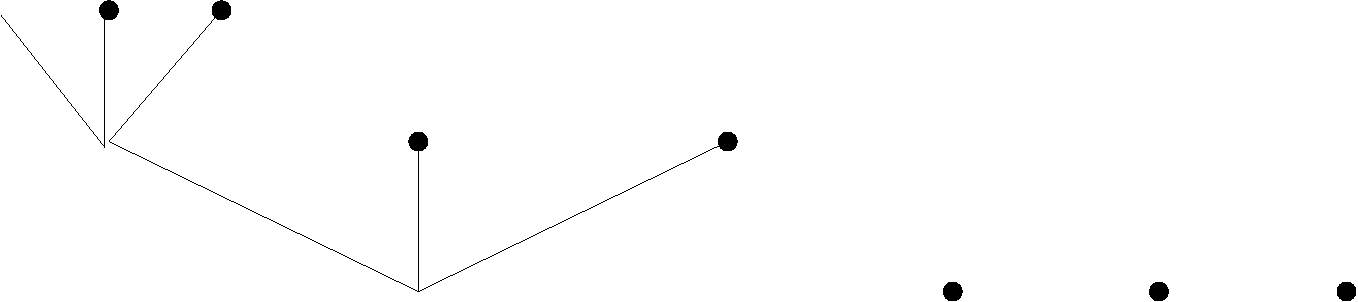
\includegraphics[width=0.5\textwidth]{indep.pdf}
\caption{Non-generating independent set~$P\subset\rmC^+_{A}[4]$ with~$|A|=3$ and~$|P|=7$ with most possible elements of height 0, then of height 1, etc. In this case, we see that~$h_{4,7,1}=2$ while~$h_{4,7,2}=3$.}
\label{fig:indep}
\end{figure}
\end{proof}



Note that we have defined the height~$h_{r,k,N}$ as the height such that there are at least~$N$ elements~$y$ of that height  with~$P\cup \{y\}$ still an independent set of cardinality~$k+1$. If we want~$P\cup \{y\}$ to be {\em non-generating}, and hence again defining a simplex of~$\rmT^\infty_r$, we need~$N\ge 2$. 


\begin{proof}[Proof of Proposition~\ref{contract1}]
We will show that, for all~$k\ge 0$, all maps~$\rmS^k\to\rmT_r^\infty$ from spheres into the space~$\rmT_r^\infty$ are null-homotopic. 
Let us be given a map~$f\colon \rmS^k\to\rmT_r^\infty$. From \cite{Zeeman}, we can assume that the sphere~$\rmS^k$ comes with a triangulation such that the map~$f$ is simplicial. 
Let~$v_i$ be the number of simplices of dimension~$i$ is this triangulation of the sphere, and 
let~$v=v_0+\dots+v_k$ be the total number of simplices of all dimensions of that triangulation. In particular, this triangulation has~$v_0\le v$ vertices. Let \hbox{$N=v+2$} and~$h=h_{r,k,N}$ be the corresponding height obtained in Lemma~\ref{lem:height}. We will start by showing that the map~$f$ is homotopic to a map whose image only contains vertices of height at least~$h$ in~$\rmT_r^\infty$, and at most~$v$ of them: we will progressively retriangulate the sphere, and the new triangulation at all time will still have at most~$v$ vertices. 

We call a simplex of the sphere~$\rmS^k$~{\it bad} for~$f$ if all of its vertices are mapped to vertices in~$\rmT_r^\infty$ that have height less than~$h$.
%If there is a bad simplex for~$f$ with respect to the given triangulation of the sphere, then we will see that we can find a homotopy from~$f$ to a map that is simplicial with respect to another triangulation of the sphere that still has at most~$v$ vertices and that has fewer~bad simplices. 
We will modify~$f$ by removing the bad simplices inductively starting by those of highest dimension. 
So let~$\sigma$ be a bad simplex of maximal dimension~$p$ among all bad simplices. We will modify~$f$ and the triangulation of the sphere in the star of that simplex in a way that does not add any new bad simplex. In the process, we will increase the number of vertices by at most~$1$, and not at all if~$\sigma$ was a vertex. 
This implies that, after doing this for all bad simplices, we will have increased the number of vertices of the triangulation of the sphere by at most~$v_1+\dots+v_k$. As the sphere originally had~$v_0$ vertices, at the end of the process its new triangulation will  have at most~$v=v_0+v_1+\dots+v_k$ vertices (as we never introduced any new bad simplices, so only bad simplices of the original triangulation affect that number). There are two cases:

{\em Case~$p=k$.} If the bad simplex~$\sigma$ is of the dimension~$k$ of the sphere~$\rmS^k$, then its image~$f(\s)$ is a non-generating independent subset of~$\rmC_{A}^+[r]$. Because it is non-generating, we can choose~$y\in \rmC_A^+[r]$ that has height at least~$h$ and that is not a descendant of any vertex of~$f(\s)$ and still, together with~$f(\s)$, gives a non-generating independent subset. As the union~$f(\sigma)\cup\{y\}$ is again a simplex of~$\rmT_r^\infty$, we can add a vertex~$a$ in the center of~$\s$, replacing~$\s$ by~$\partial \s*a$ and replace~$f$ by the map~$(f|_{\partial\s})*(a\mapsto y)$ on~$\partial\sigma*a$. This map is homotopic to~$f$ through the simplex~$f(\s)\cup \{y\}$. We have added a single vertex to the triangulation. Because~$y$ has height~$h$, we have not added any new bad simplex, and we have removed one bad simplex, namely~$\s$. 

{\em Case~$p<k$.} If the bad simplex~$\sigma$ is a~$p$--simplex for some~$p<k$, by maximality of its dimension, the link of~$\sigma$ is mapped to vertices of height at least~$h$ in the complement of the free~$A^*$--set~$\rmC_A^+(f(\s))$ generated by~$f(\sigma)$. %These must lie in the the~$A^*$-invariant subset generated by the complement of the minimal basis containing~$f(\s)$. 
The simplex~$\s$ has~$p+1$ vertices whose images form an independent subset of~$\rmC_{A}^+[r]$ of cardinality at most~$p+1\leqslant k$.
By our choice of $h$, there are at least~$N= v+2$ vertices~$y_1,\dots,y_N$ of height~$h$ %in the complement of~$\rmC_{A}^+(f(\s))$, that is vertices 
such that each~$f(\s)\cup\{y_i\}$ still forms an independent set. 
Consider the~$A^*$--set 
$$\rmC_A^+(y_1)\sqcup\dots\sqcup\rmC_A^+(y_N)\ \subset \rmC_A^+[r].$$
As there are fewer vertices in the link than in the whole sphere, and the whole sphere has at most~$v$ vertices, by the pigeonhole principle, the vertices of~$\Link(\s)$ are mapped to at most~$v$ of the subsets~$\rmC_A^+(y_i)$. As~$N=v+2$, 
there are at least two of the above vertices~$y_i$ and~$y_j$ of height~$h$  such that no vertex of the link is mapped to any of their descendants~$\rmC_A^+(y_i)\sqcup\rmC_A^+(y_j)$. As these vertices are 
to start with independent of~$f(\s)$, it follows that for any simplex~$\tau$ of~$\Link(\s)$, the union~$f(\tau)\cup f(\s)\cup\{y_i\}$ is an independent set. Moreover this set is also non-generating because~$y_j$ is still independent of it. Hence  each~$f(\tau)\cup f(\s)\cup\{y_i\}$ forms a simplex of~$\rmT_r^\infty$. We can then replace~$f$ inside the star
\[
\Star(\s)=\Link(\s)*\s\simeq \rmS^{k-p-1}*\rmD^p
\]
by the map~$(f|_{\Link(\s)})*(a\mapsto y_i)*(f|_{\partial \s})$ on 
\[
\Link(\s)*a*\partial\s\simeq \rmS^{k-p-1}*D^0*\rmS^{p-1}.
\]
which agrees with~$f$ on the boundary~$\Link(\s)*\partial\s$ of the star, and is homotopic to~$f$ 
through the map~$(f|_{\Link(\s)})*(a\mapsto y_i)*(f|_{\s})$ defined on 
\[
\Link(\s)*a*\s\simeq \rmS^{k-p-1}*D^0*\rmD^p.
\] 
Now~$\Link(\s)*a*\partial(\s)$  has exactly one extra vertex compared to the star of~$\s$, unless~$\s$ was just a vertex, in which case its boundary is empty, and it has the same number of vertices.
As~$y_i$ has height~$h$, we have not added any new bad simplices. Hence we have reduced the number of bad simplices by one because~$\s$ was removed. 

By induction, we can now assume that there are no bad simplices for~$f$ with respect to a triangulation with at most~$v$ vertices. With this assumption, we can 
cone off~$f$ just as we coned off the links in the above argument:  We have more than~$N=v+2$ vertices of height~$h$ in~$\rmT_r^\infty$, and at most~$v$ vertices in the sphere. These vertices are mapped to vertices of height at least~$h$, that is to descendants of the vertices of height~$h$. By the pigeonhole principle, we know that there are at least two vertices~$y_i$ and~$y_j$, of height~$h$ such that no vertex of the sphere is mapped to any of their descendants. Hence we can cone off the sphere using~$\{y_i\}$. Indeed, this~$\{y_i\}$ is disjoint and independent from the set~$f(\sigma)$ for every simplex~$\s$ of the sphere, ensuring that the union~$f(\s)\cup\{y_i\}$ still forms an independent set, and any such set is non-generating because~$y_j$ is independent of it. Hence every~$f(\s)\cup\{y_i\}$ defines a simplex of~$\rmT_r^\infty$ and we can cone off the sphere by adding a single vertex mapped to~$y_i$. 
\end{proof}


\begin{proof}[Proof of Proposition~\ref{contract2}]
Consider a map~$f\colon\rmS^k\to\rmU_r^{\infty}$. Again we can assume that it is simplicial for some triangulation of the sphere~$\rmS^k$. We will show that there is a homotopy from~$f$ to a map that lands inside~$\rmT_r^\infty$. This will prove the result by Proposition~\ref{contract1}. 

We will, just like in the previous proof, modify~$f$ by a homotopy on the stars of the {\it bad} simplices in~$\rmS^k$, namely those whose vertices are all mapped to~$\rmU_r^\infty\backslash\rmT_r^\infty$. We will show how to reduce their number one by one, so that the result follows by induction.

Let~$\s$ be a bad simplex of maximal dimension, say~$p$, in the sphere~$\rmS^k$. By maximality, the link of~$\s$ is mapped to
%$\rmT_r^\infty\cap\operatorname{Star}(f(\s))$, which itself equals
~\hbox{$\rmT_r^\infty\cap\Link(f(\s))\subset \rmU_r^\infty$}.  
%as the vertices of~$f(\s)$ are mapped to~$\rmU_r^\infty\setminus\rmT_r^\infty$. 
We now argue that the intersection~\hbox{$\rmT_r^\infty\cap\Link(f(\s))$} is isomorphic to~$\rmT_{q}^\infty$ for some~$q\geqslant1$.

The simplex~$f(\sigma)$ is a collection of disjoint subsets of~$\rmC_{A}^+[r]$ that together form a non-generating independent subset~$P\in \calI_0[r]$. By Lemma~\ref{lem:minexp}, there exists a least expansion~$E$ of~$[r]$ containing~$P$, and because~$P$ is non-generating, the set~$E\minus P=Q$ has cardinality~$q\ge 1$. 
We claim that~$\rmT_r^\infty\cap\Link(f(\s))$ is isomorphic to~$\rmT_q^\infty$. 
To write a map, we first pick a bijection~$\la\colon[q]\to Q$.  Then~$\la$, together with the inclusion~$Q\subset\rmC_A^+[r]$ induces a map 
$$\hat\la\colon \rmC_A^+[q] \rar \rmC_A^+[r]$$
which in turn induces a map 
$$T(\hat \la)\colon \rmT_q^\infty \rar \rmT_r^\infty$$
defined on vertices by~$T(\hat\la)(y)=\hat\la(y)$. 
Indeed, the map~$\hat\la$ respects independency of subsets, which shows that~$T(\hat\la)$ is simplicial. 
Now note that any simplex of~$\rmT_r^\infty$ in the image of~$T(\hat \la)$ lies in the link of~$f(\s)$ because it necessarily is an independent strict subset of some expansion of~$Q$, and hence is independent of~$f(\s)$, and, together with $f(\s)$, non-generating. On the other hand, any simplex~$\tau$ of~$\rmT_r^\infty\cap\Link(f(\s))$ is defined by an independent set~$R$ such that~$R\cup P$ is (non-generating) independent. Let~$E'$ be some expansion of~$[r]$ containing~$R\cup P$. By minimality of~$E=Q\cup P$, we must have that~$E'$ is an expansion of~$E$ and hence that~$R$ lies in some expansion of~$Q$. It follows that~$\tau$ was actually in the image of~$T(\hat \la)$. 
Hence~$T(\hat\la)$ defines an isomorphism~\hbox{$\rmT_q^\infty\cong \rmT_r^\infty\cap\Link(f(\s))$}. 



Let us consider the restriction of the map~$f$ to the star of the simplex~$\s$. Since we are working inside a~$k$-sphere, we have
\[
\Star(\sigma)\cong\Link(\sigma)*\sigma\cong \rmS^{k-p-1}*\sigma.
\]
The simplicial complex~$\rmT_{q}^\infty$ is contractible by Proposition~\ref{contract1}. As the link of~$f(\s)$ is mapped into the intersection~\hbox{$\rmT_r^\infty\cap\Link(f(\s))$}, which is isomorphic to~$\rmT_q^\infty$, we can extend the map from the link to a map~\hbox{$g\colon\rmD^{k-p}\to \rmT_r^\infty\cap\Link(f(\s))$}. 
Using such a map, the restriction of the map~$f$ to the star of the simplex~$\s$ can be extended to get a map~\hbox{$\hat f=g*f\colon\rmD^{k-p}*\s\to\rmU_r^\infty$} on the ball~$\rmD^{k-p}*\s$. 
%with~$D^{k-p}$ mapped to~$T_{q}^\infty$. 
This extension defines a homotopy on the star of~$\s$ in~$\rmS^k$, relative to the boundary link, from the restriction of~$f$ to a map with strictly fewer bad simplices: 
The new map~$g*f\colon\rmD^{k-p}*\partial\s\to\rmU_r^\infty$ has fewer old bad simplices, because~$\s$ has been removed, and 
there are no new bad simplices, because new simplices are joins of faces of~$\partial\s$ and simplices in the disc~$\rmD^{k-p}$, but the latter is mapped to good vertices. The result follows by induction.  
\end{proof}


%%%
